\section{}
\textit{A person drops 3 aluminum balls of diameters 2 mm, 4 mm, and 10 mm into a tank filled with glycerin at 22°C ($\mu = 1 \, \text{kg} \cdot \text{m/s}$), and measured the terminal velocities to be 3.2 mm/s, 12.8 mm/s, and 60.4 mm/s, respectively. The measurements are to be compared with theory using Stokes law for drag force acting on a spherical object of diameter $D$ expressed as $F_D = 3\pi\mu VD$ for $Re \ll 1$. Compare experimental velocities values with those predicted theoretically.}

\begin{figure}[H]
    \centering
    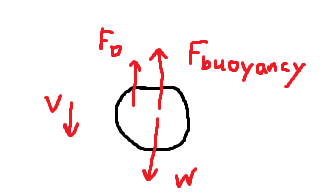
\includegraphics[width=0.6\textwidth]{Questions/Figures/Q1 FBD.png}
    \caption{Free body diagram of a sphere in a fluid.} 
    \label{fig:Q1 FBD}
\end{figure}
Since at terminal velocity, the acceleration is zero, by Newton's Second Law,
\begin{align*}
    w &= F_D + F_{\text{buoyancy}} 
\end{align*}
By Stokes' Law, 
\begin{align*}
    \frac{\pi}{6}D^3\rho_{\text{aluminum}}g &= 3\pi\mu VD + \frac{\pi}{6}D^3\rho_{\text{glycerin}}g
\end{align*}
Rearranging for $V$,
\begin{align*}
    V &= \frac{D^2}{18\mu}\left(\rho_{\text{aluminum}} - \rho_{\text{glycerin}}\right)g
\end{align*}
Assuming pure aluminum, $\rho_{\text{aluminum}} = 2702 \, \text{kg/m}^3$, and at 22°C $\rho_{\text{glycerin}} = 1263$ \cite{cengel_thermodynamics:_2024}. Substituting these values into the equation, we can calculate the theoretical terminal velocities for each diameter, shown in Table \ref{tab:Q1}.

The error is calculated as
\begin{align*}
    \text{Error} &= \frac{|V_{\text{exp}} - V_{\text{theo}}|}{V_{\text{theo}}}\times 100\%
\end{align*}

The Reynolds number is calculated as
\begin{align*}
    \text{Re} &= \frac{\rho_{\text{glycerin}}VD}{\mu}
\end{align*}

The agreement between the theoretical and experimental terminal velocities is good for the 2 mm and 4 mm diameters, with relative errors of 2.01\%. However, the relative error for the 10 mm diameter is 22.98\%. This is likely due to the Reynolds number being a magnitude higher than the 4 mm diameter. As diameter increases, the Reynolds number increases, and the assumption that $Re \ll 1$ will become less accurate.

\begin{table}[H]
    \centering
    \caption{Comparison of Theoretical and Experimental Terminal Velocities}
    \label{tab:Q1}
    \begin{tabular}{C{0.15\textwidth}C{0.15\textwidth}C{0.15\textwidth}C{0.15\textwidth}C{0.15\textwidth}}
    \toprule
    Diameter & Theorerical Terminal Velocity, $V$ & Experimental Terminal Velocity & Relative Error & Reynolds Number \\
    (mm) & (mm/s) & (mm/s) & (\%) &  \\
    \midrule
    2 & 3.14 & 3.2 & 2.01 & 0.008 \\
    4 & 12.55 & 12.8 & 2.01 & 0.032 \\
    10 & 78.43 & 60.4 & 22.98 & 0.198 \\
    \bottomrule
    \end{tabular}
\end{table}